
\chapter{Background}
\label{chap:background}

\section{Related Work}

\subsection{EEG Classification Methods}

A wide range of methods have been proposed to detect patterns in brain activity corresponding to health related events, cognitive activities, and specific mental states. The goal of these methods is to extract information from raw EEG signals corresponding to high-level brain states, which enables advanced diagnostic techniques, monitoring, and brain–computer interfaces.

Classical machine learning algorithms formed the basis of early EEG classification systems combined with manually designed feature extraction pipelines \cite{8972542}. These methods apply traditional classifiers to the extracted features, such as k-nearest neighbors, naive Bayes, support vector machines, decision trees, and random forests \cite{technologies10040079}. The main problem with these models is their dependence on feature extraction quality and their limited generalisation ability to larger datasets.

Deep learning-based classification methods have become popular in recent years. The most commonly used model family in the industry is convolutional neural networks (CNNs), which use temporal and spatial convolutions, as in EEGNet \cite{Lawhern_2018}, ShallowFBCSPNet \cite{EEGInceptionERP}, and EEGInceptionERP \cite{EEG-Inception}. Purely CNN models like EEGNeX \cite{CHEN2024105475} are still able to achieve SOTA performance on many benchmark problems. 

Recurrent neural networks (RNNs) combined with CNNs are able to both learn spatial feature extraction and perform sequence modeling. Hybrid CNN-LSTM \cite{inproceedings} models provide strong foundation and enable improved classification performance. 

Attention-based models further improve EEG analysis with the ability to capture long-range dependencies. Architectures like EEGConformer \cite{Conformer} and EEGPT \cite{wang2024eegpt} have delivered promising results in classification tasks where temporal patterns play a significant role.

The introduction of graph neural networks (GNNs) has also gained attention in the field, but these methods are still relatively new, and their effectiveness and applicability remain not fully established.

Despite the strong results of deep learning-based methods, their performance highly depends on the amount of labeled data, making classical machine learning approaches remain competitive in many real-world scenarios.

\subsection{EEG Artifact Detection}

EEG recordings often contain artifacts, which are characteristic signal patterns corresponding to different sources. Some earlier works focused on the suppression or removal of these artifacts, mainly by using filtering techniques \cite{QUAZI2017401} and developing strong preprocessing pipelines \cite{RICOOLARTE2025103702}. Recent studies even apply deep learning techniques on synthetic and real datasets with the goal of complete artifact removal \cite{FERNANDEZDERETANA2025152}\cite{app15094953}.

Deep learning techniques become SOTA solutions for classification tasks defined by benchmark artifact datasets. The TUH EEG Artifact Corpus (TUAR) \cite{9353647} provides large number of EEG recordings on which many models and methods are tested. There are earlier works that introduce both single label and multi label classification setups using the TUAR dataset \cite{TUAR}.

Studies have built upon the TUAR benchmark, developing new models \cite{TUAR2} and exploring energy-efficient monitoring techniques for epilepsy detection \cite{energy}, yet relatively few works have focused on classifying rare artifacts and solving challenges caused by class imbalance.

Additionally, artifacts are also explored with the aim of improving seizure detection models \cite{inproceedings}, due to the temporal and morphological similarities of seizure and certain artifact characteristics, while other studies focus on data splitting techniques to simulate realistic clinical environments.

\subsection{Data Augmentation Techniques}

The introduction of deep learning techniques and their success in EEG related tasks has shifted the focus to data augmentation techniques. Due to the large data requirements of these models, augmentations that increase the variance of the dataset have proven useful for problems with low samples-to-features ratio \cite{LASHGARI2020108885}.

Some works evaluate the effects of specific augmentation methods, such as pink and Gaussian noise addition \cite{pink} or time–frequency transformations \cite{WANG2025113074}, while others focus on developing stronger data augmentation pipelines for a targeted use case like epilepsy detection \cite{epi}. These solutions have become an essential component of most EEG related deep learning approaches. 

In recent years, generative models proved to be the next step in the field of EEG augmentation as well by introducing fully synthetic data generation techniques. Using generated data not only increases variance in the dataset, but also helps address data imbalance problems. Recent works have successfully improved overall performance with class specific data generation \cite{Fan_2020}.

Most studies have used generative adversarial networks (GANs) for data generation \cite{gan2}, but diffusion-based methods have emerged as a new candidate for such tasks \cite{puah2025}. Both models have been used in many studies for enhancing and expanding existing smaller datasets, while relatively few have focused on artifact specific data generation.

A related study compared GAN and diffusion models for EEG artifact synthesis, but its main objective was to evaluate class-conditional consistency rather than to improve classification performance using the generated data, and the diffusion model operates directly on the raw signal instead of a latent space \cite{arasu2025}.

While recent works highlight growing importance of data oriented approaches in EEG analysis, they also present a gap in the systematic evaluation of augmentation strategies for artifact classification tasks.

\newpage

\section{Dataset}

\subsection{TUAR Dataset Description}

The dataset used was the TUH EEG Artifact Corpus (TUAR) \cite{9353647}. This dataset is a subset of the Temple University Hospital EEG Corpus (TUH EEG), a large-scale collection of clinical EEG recordings gathered during routine patient care at Temple University Hospital. The TUH EEG dataset was created to support research in machine learning and deep learning methods, EEG analysis and classification. TUAR is a specialised subset containing common artifacts that occur in clinical EEG measurements. This labeled dataset enables supervised learning methods to be trained for artifact detection and classification. 

There are three different channel configurations in the TUAR dataset that correspond to different ways of referencing and organizing the EEG electrodes. All three datasets use the same electrode positions based on the Transverse Central Parietal (TCP) configuration, so the electrode names and positions are consistent. The difference between them is how the signals are referenced. The one with the most recordings is the Averaged Reference (AR) configuration where the signals are re-referenced to the average of all electrodes. There is a modified Averaged Reference Alternate (AR-A) configuration setup and a Linked Ears (LE) configuration in which the signals are referenced to linked earlobes or mastoid electrodes. For the experiments conducted in this thesis, the EEG recordings with the AR configuration were used. 

Figure~\ref{fig:electrodes} illustrates the EEG electrode layout in an AR montage. Each channel represents the potential difference between a given electrode and the average potential of all electrodes. This results in signals such as Fp1–Avg, F3–Avg, and Cz–Avg, where the common reference is the global mean across all channels.

Recordings are stored in the European Data Format (EDF), a widely used standard for electroencephalography signals. Each file follow a strict naming convention containing a subject identifier, a session number and a token number, used to split long recordings into smaller segments. All EEG files have a corresponding CSV annotation file in the same directory. The CSV file contains information for the artifact events that are present in the recording.

\begin{figure}[H]
\centering
    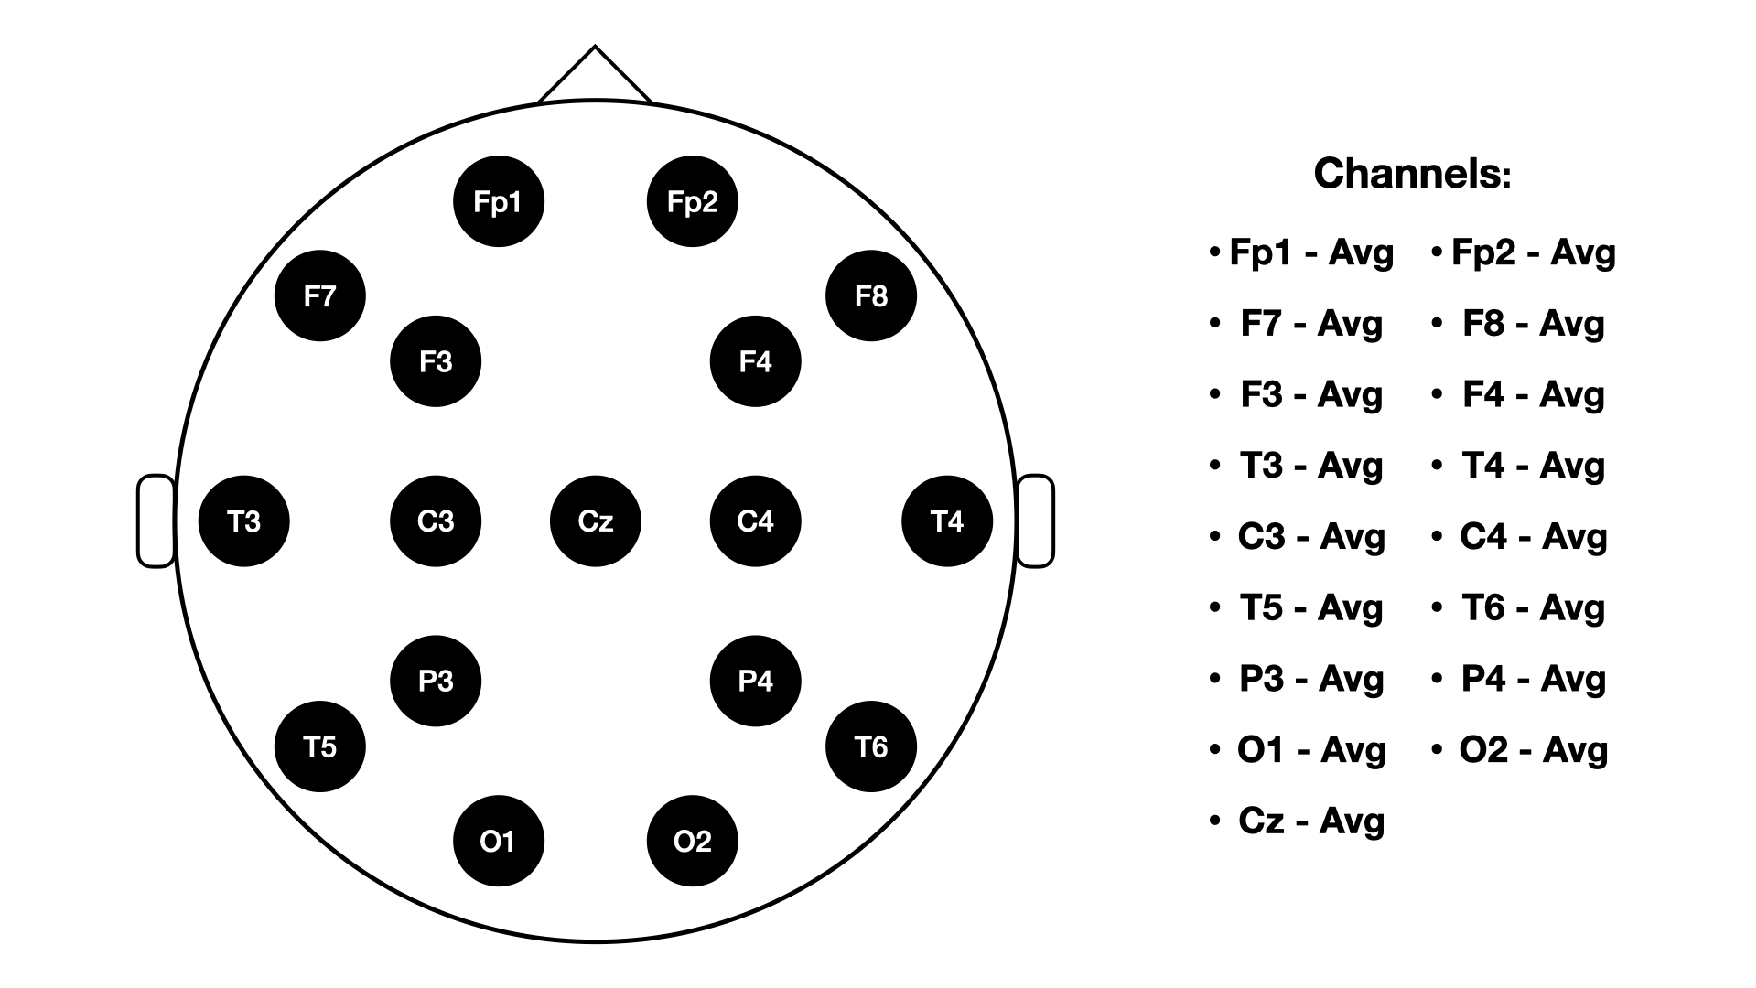
\includegraphics[width=0.8\textwidth]{images/electrodes.pdf}
    \caption{Average-referenced EEG channels across the scalp.}
    \label{fig:electrodes}
\end{figure}

\subsection{Annotation Scheme}

The annotations of the recordings were created by expert EEG annotators associated with Temple University and the Neural Engineering Data Consortium (NEDC). Each artifact event is described by a set of fields:

\textbf{channel} - The EEG channel affected by the artifact.

\textbf{start\_time} - The time, in seconds, when the artifact starts

\textbf{stop\_time} - The time, in seconds, when the artifact ends.

\textbf{label} - The type of artifact.

\textbf{confidence} - A numerical score indicating the confidence of the annotation.\\

The TUAR corpus defines a set of standard artifact classes that occur in clinical EEG recordings \cite{9353647}. Each annotated event belongs to one of the following classes:

\begin{description}

\item[\textbf{Eye movements (eyem):}] A very common artifact caused by movement of the patient’s eyes. These movements create strong signals on channels representing the frontal polar electrodes. Large spans of eye movement artifact can contribute to errors in automated seizure detection because the produced wave patterns may resemble seizure activity.

\item[\textbf{Muscle activity (musc):}] Muscle artifacts are linked to physical activity. They are quite frequent and often sudden, reflecting a state of agitation or nervousness in a patient. Their amplitude varies considerably, and their frequency is higher than 30 Hz.

\item[\textbf{Chewing (chew):}] A chewing artifact is a subset of muscle activity resulting from the tensing and relaxing of the jaw. It primarily appears on temporal channels and may show stronger activity in one hemisphere. This artifact has the characteristic high-frequency activity of muscle artifacts and commonly appears when patients move their jaw during sleep.

\item[\textbf{Shivering (shiv):}] Shivering artifact is another subset of muscle artifact that occurs when a patient shivers. It typically appears across the majority of channels. Although relatively rare, it can cause significant errors in automated analysis when present.

\item[\textbf{Electrode-related artifacts (elec):}] These artifacts are caused by issues with EEG electrodes or their connections. They include disturbances such as electrode pops, electrostatic interference, and lead artifacts, which usually appear as sudden spikes or abrupt signal changes in the affected channel.

\item[\textbf{Electrode pop (elpp):}] The electrode pop is a particular form of electrode artifact that happens as a result of a problem with a single electrode. This problem could be attributed to poor electrode attachment or air bubbles present in the conductive gel. Sometimes, the electrode pops multiple times during the recording session.

\end{description}

Segments of the EEG signal that are not annotated with any artifact label are considered \textbf{background}.

\newpage

\subsection{Dataset Analysis}

The TUAR dataset is significantly class-imbalanced, with annotation counts ranging from a few hundred to over one hundred thousand. Major classes like \texttt{musc} and \texttt{eyem} dominate, while the underrepresented minor classes contributing less than 0.1\% of the total annotations. This can result in bias toward frequent classes and weaken performance on rare artifacts. The analysis suggests the use of class weighting to compensate for the class imbalance.



\begin{figure}[H]
\centering
    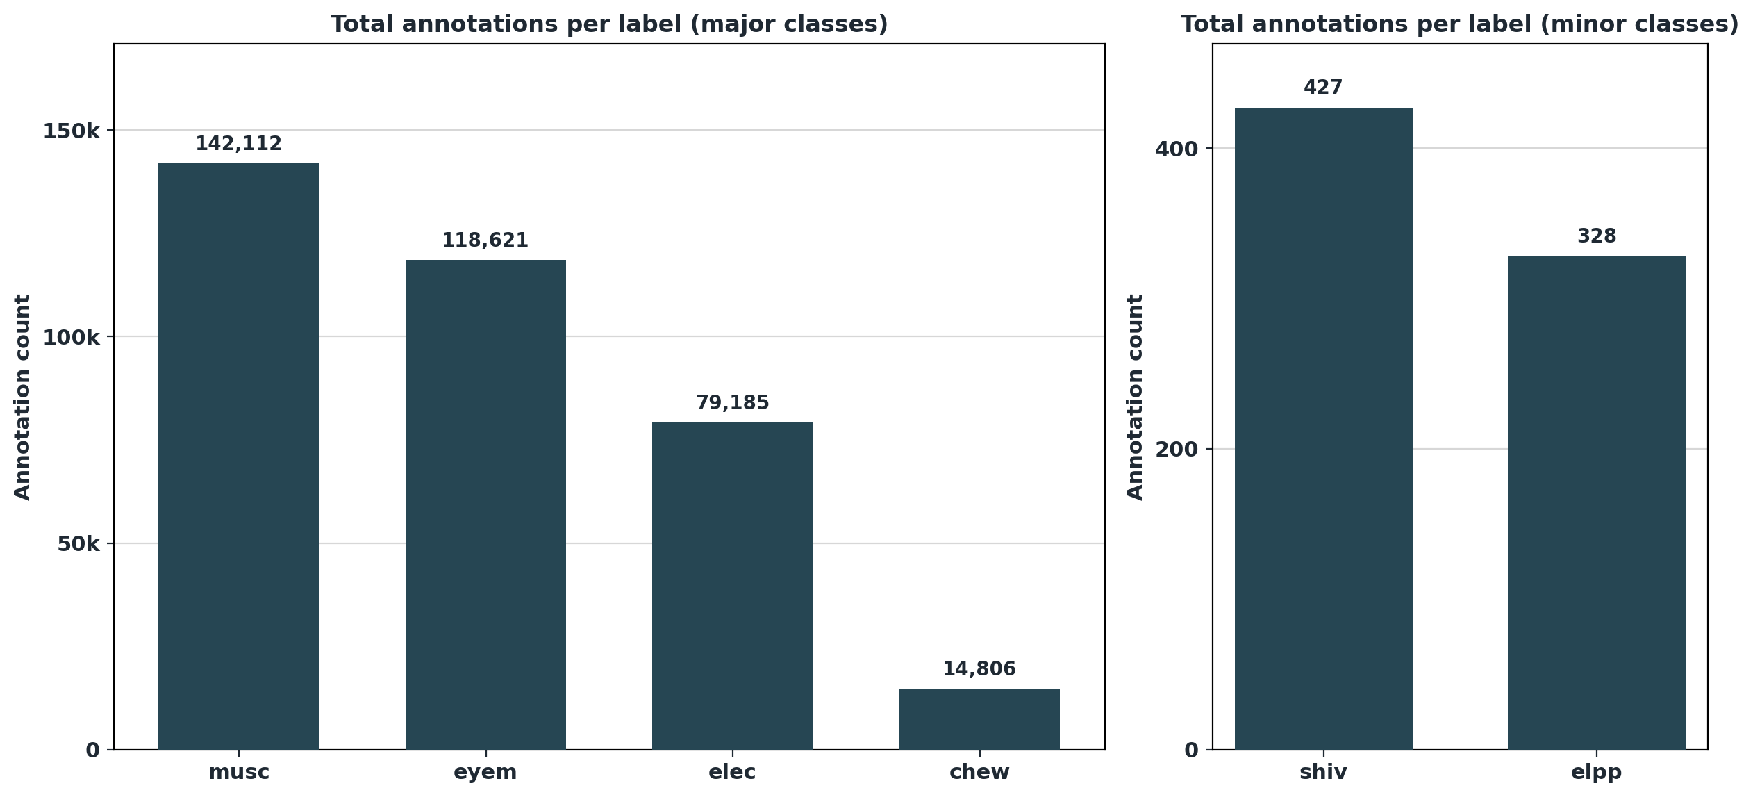
\includegraphics[width=0.9\textwidth]{images/class_annotation_counts_total.pdf}
    \caption{Total number of annotations per class in the TUAR dataset, highlighting class imbalance between major and minor categories.}
    \label{fig:annotation_counts}
\end{figure}

Balanced class distribution across splits was produced using the described dataset splitting strategy. Figure~\ref{fig:class_distribution} compares how much time each artifact class occupies in each split and in the whole dataset. It also shows that the recordings are densely annotated. 

Among the major classes, \texttt{musc} consistently represents the largest share, accounting for approximately one-fifth of the total recording time across all splits. In most classes only minor variations between splits can be observed, with the exception of \texttt{shiv}, where most of the recording containing the artifact ended up in the train split. This is due to the fact that only a small number of recordings contain \texttt{shiv}. As a result of the patient-wise splitting strategy, this distribution represents the closest achievable ratio to the target split proportions. In conclusion, the resulting distribution across splits provides a reliable basis for model evaluation.

\begin{figure}[H]
\centering
    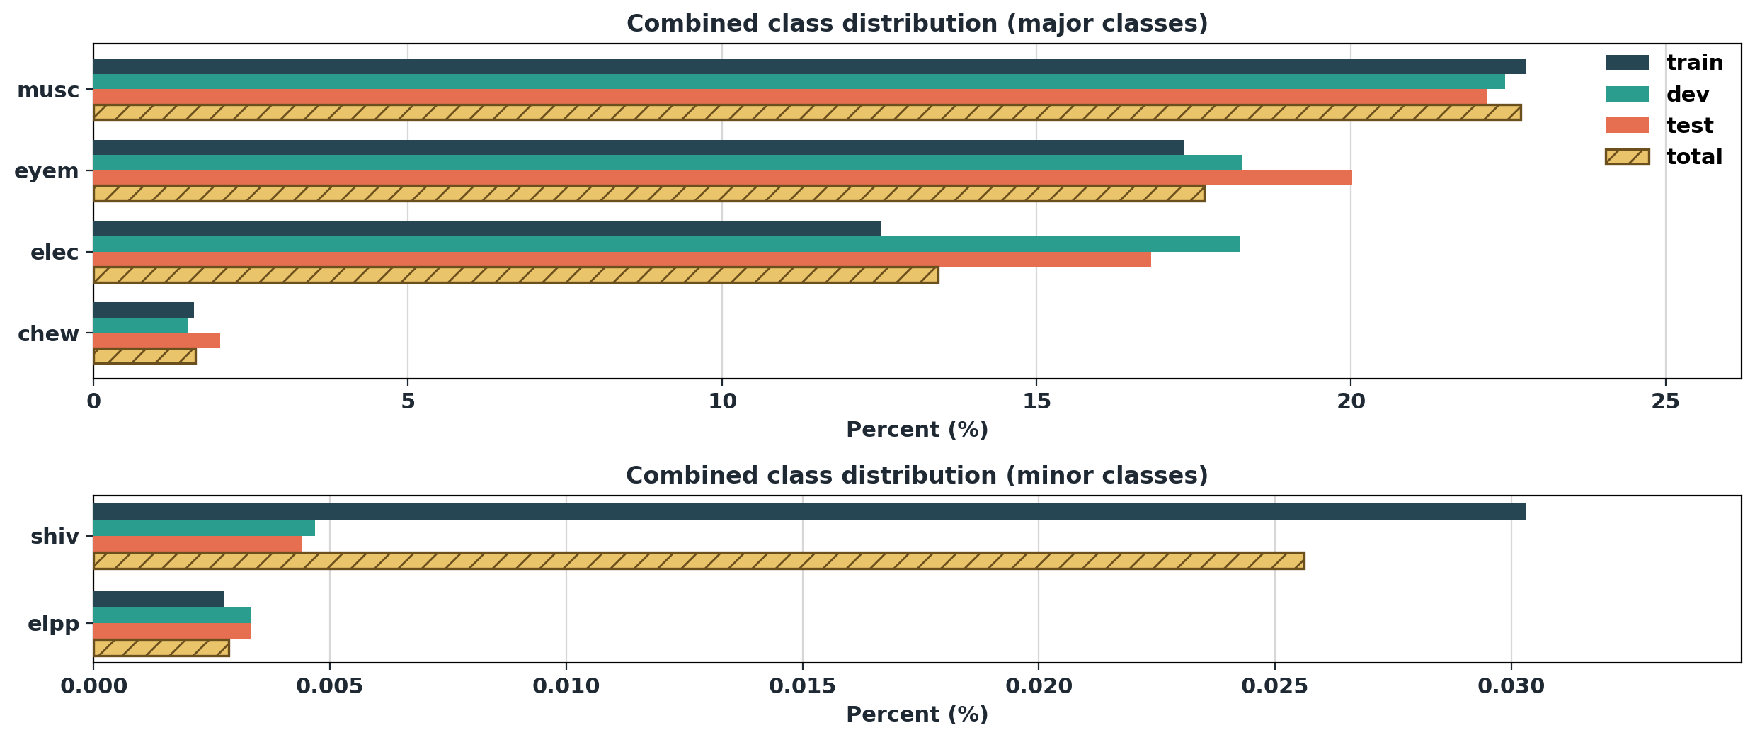
\includegraphics[width=0.9\textwidth]{images/class_distribution_pct_total_time_combined.pdf}
    \caption{Distribution of artifact classes across dataset splits based on recording time.}
    \label{fig:class_distribution}
\end{figure}

The distribution of annotation durations is shown in Figure~\ref{fig:length_distribution_3x2}. The majority of annotations are short, with most labeled segments lasting around 1 second, while some annotated sequences extend to several minutes. This highlights the uneven distribution of artifacts, where short events dominate, while longer occurrences remain relatively rare.

\begin{figure}[H]
\centering
    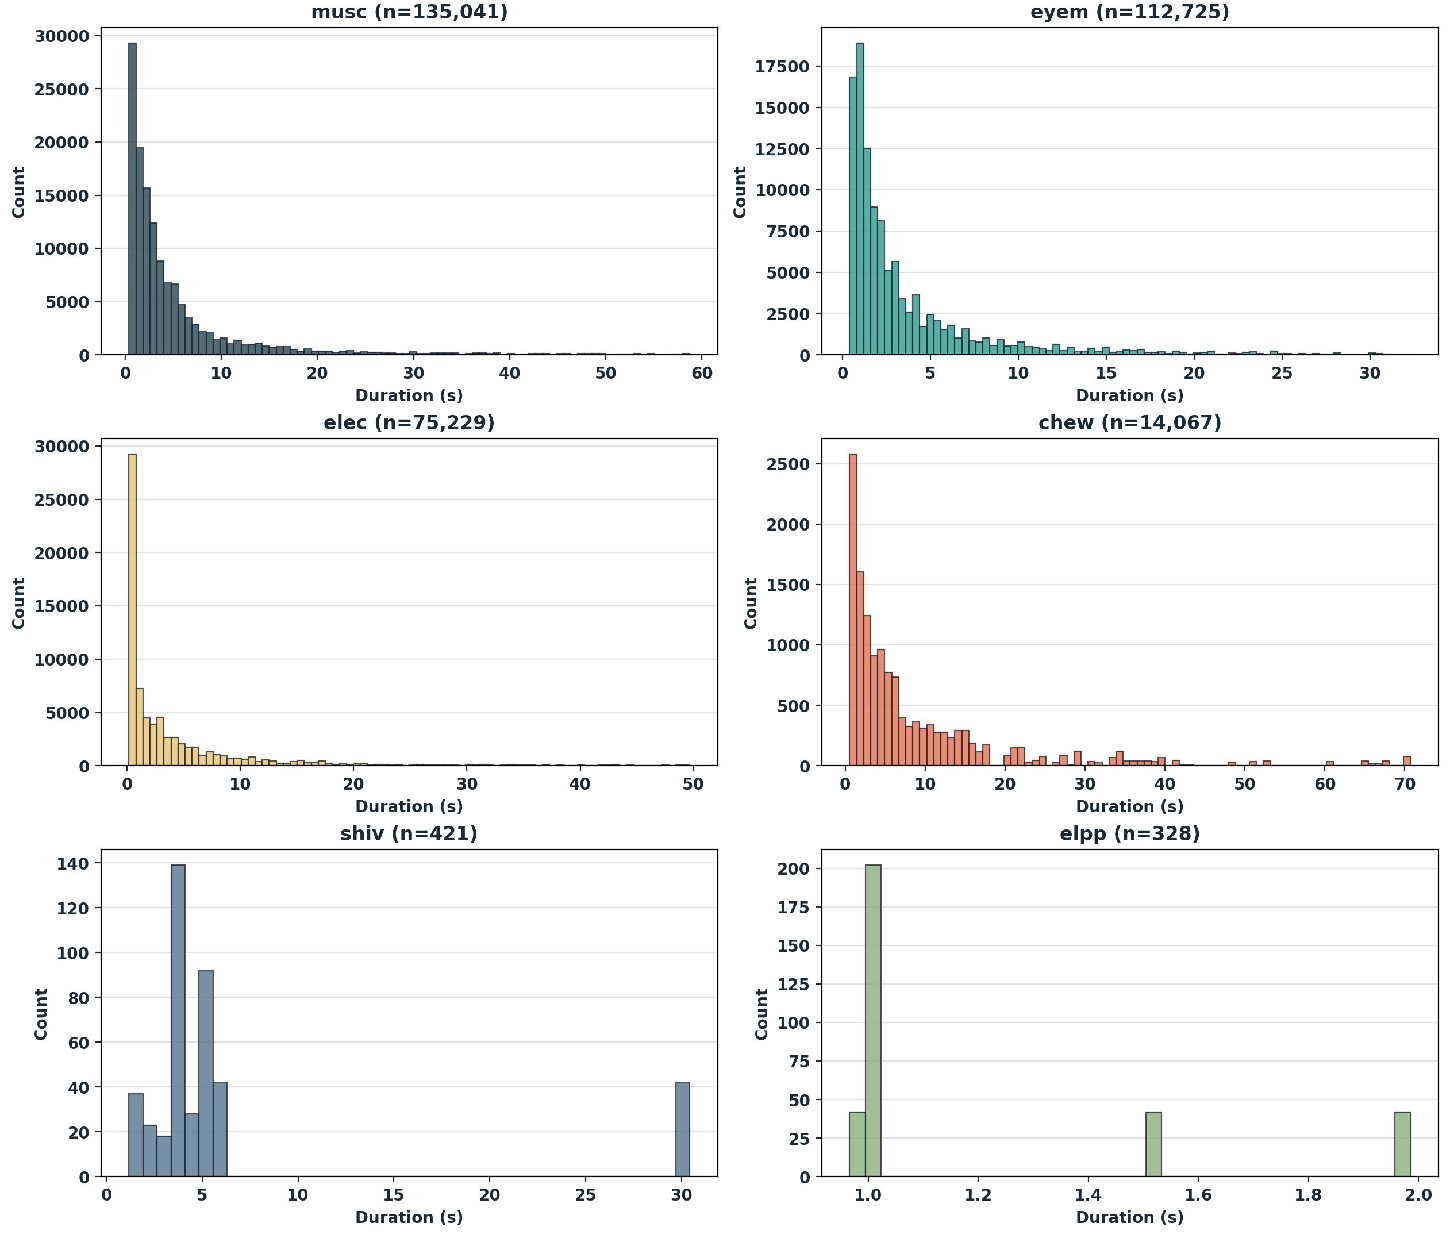
\includegraphics[width=0.9\textwidth]{images/class_annotation_length_distribution_3x2.pdf}
    \caption{Distribution of annotation durations for each artifact class. Extreme outliers are not shown for clarity.}
    \label{fig:length_distribution_3x2}
\end{figure}

The window segments of the recordings are only partially covered by annotations in most cases. This is because the majority of the artifact events are short, resulting in annotations that occupy only a fraction of a given window. However, in cases of longer artifacts, the whole segment can be covered. 

Figure~\ref{fig:eeg_window} illustrates a 4 second long window visible containing an artifact in the middle. The artifact is labeled \texttt{musc} and simultaneous present on across all channels. Outside the artifact, smoother, lower-amplitude fluctuations are present, which are characteristic of typical background EEG activity. This example illustrates how artifacts can affect multiple channels simultaneously, producing characteristic patterns in the EEG signal. 


\begin{figure}[H]
\centering
    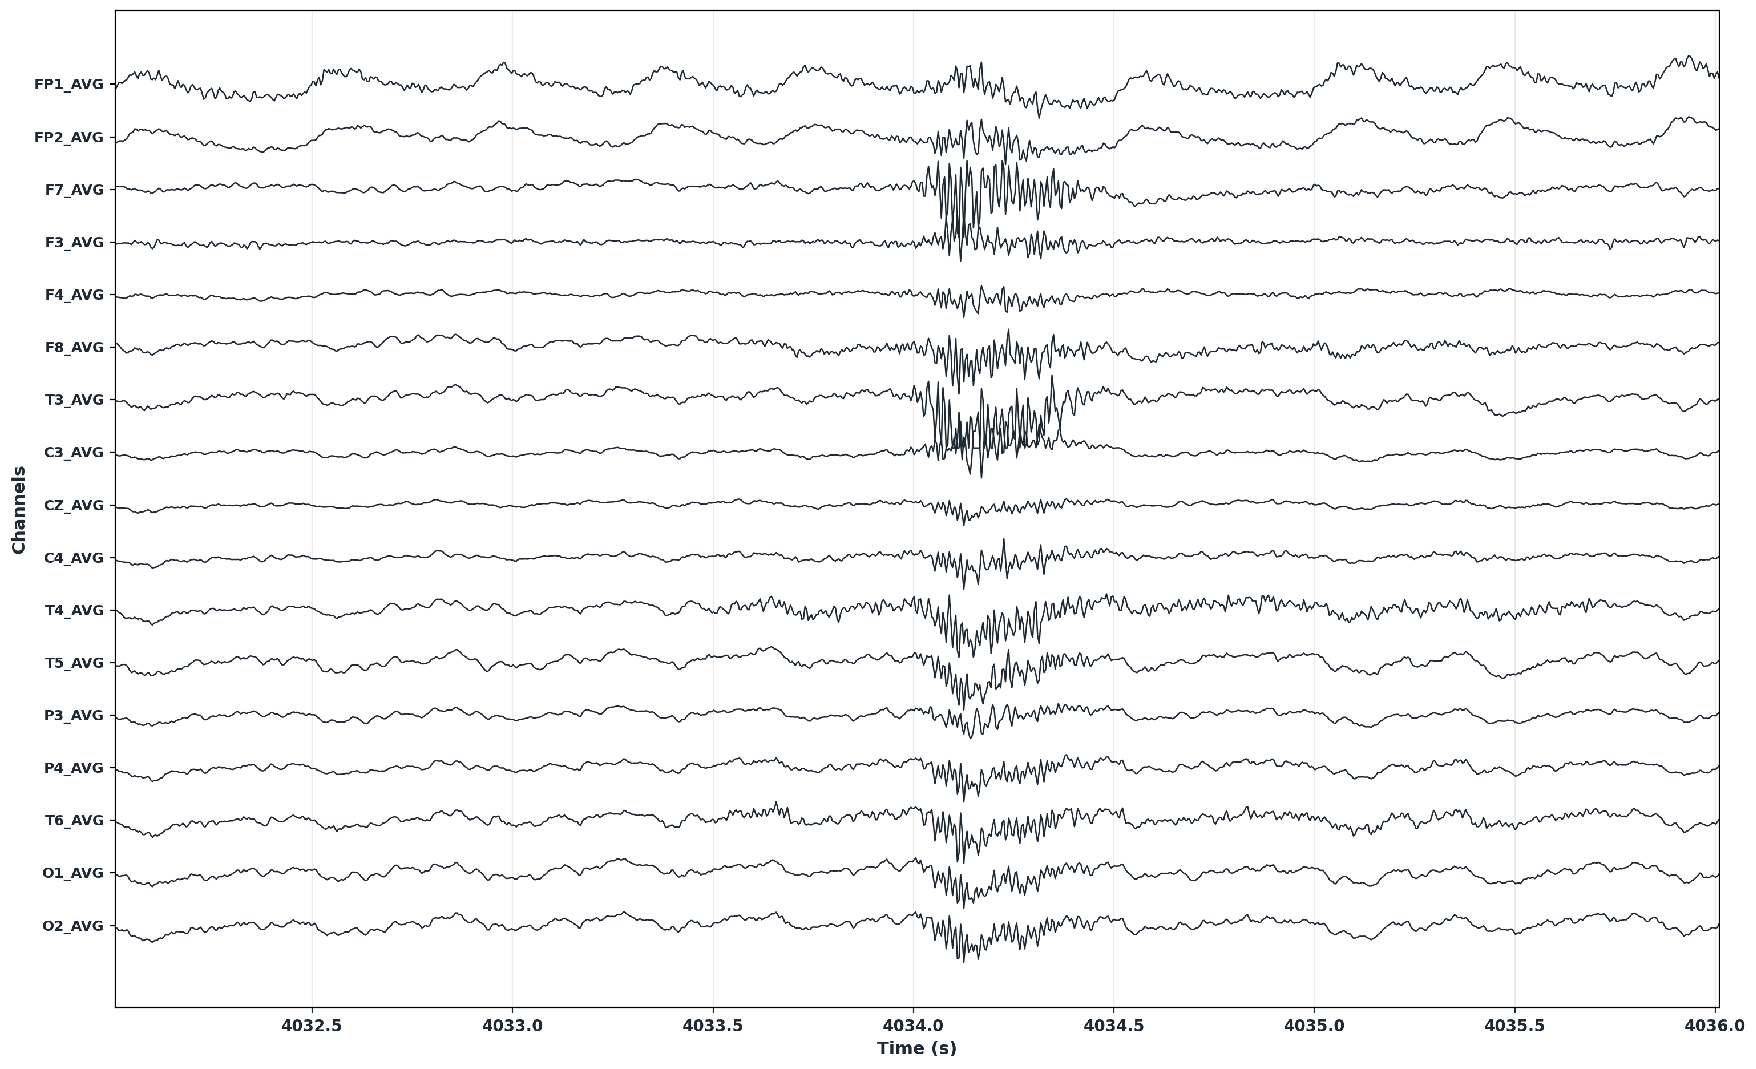
\includegraphics[width=0.9\textwidth]{images/artifact_eeg_window_4s_musc_notitle.pdf}
    \caption{Example of a 4-second EEG segment showing a \texttt{musc} artifact.}
    \label{fig:eeg_window}
\end{figure}

\section{Baseline Data Augmentation Methods}

In this section the baseline data augmentation methods are introduced. The proposed method is compared against these as described in Chapter \ref{chap:methodology} and analysed in Chapter \ref{chap:results}. The set of baseline augmentations contains six commonly used nongenerative augmentation and one WGAN-based generative method. The effects of these augmentations on classification performance are measured both separately and combined using multiple EEG classification models.

\subsection{Additive Gaussian and Pink Noise Augmentation}

Two noise-based data augmentation methods were selected: Gaussian (white) noise augmentation and pink noise augmentation, both widely used in EEG signal classification. The goal of these augmentations is to add controlled stochastic variations to the signal while preserving its structure. This reduces sensitivity to noise and reduces overfitting to the training data.

During both gaussian and pink noise augmentation, $\mathrm{RMS}_{\text{signal}}$ is computed per channel for each window $x \in \mathbb{R}^{C \times T}$, where $C$ and $T$ denote the number of EEG channels and the number of time samples in the window.

\[
\mathrm{RMS}_{\text{signal}} = \sqrt{\frac{1}{T} \sum_{t=1}^{T} x_t^2}
\]

The signal-to-noise ratio (SNR) defined in decibels is converted into a linear ratio and then used to calculate the target amplitude of the noise relative to the original signal.

\[
\mathrm{SNR}_{\text{linear}} = 10^{\mathrm{SNR}_{\text{dB}} / 20}
\]

\[
\mathrm{RMS}_{\text{noise}} = \frac{\mathrm{RMS}_{\text{signal}}}{\mathrm{SNR}_{\text{linear}}}
\]


The Gaussian augmentation assembles the noise signal by generating samples from a standard normal distribution. It is then scaled accordingly using the signal-to-noise ratio and the scaled noise is added to the original EEG signal.

Instead of generating noise directly in the time domain, the pink noise augmentation uses a frequency-domain representation. First, a random spectrum is created and then reshaped to follow a distribution $1/f$ by scaling each frequency component inversely with the square root of its frequency. The spectrum is transformed back to the time domain with the inverse Fourier transform that results in a temporally correlated noise signal. The signal is normalised, scaled using the signal-to-noise ratio, and added to the original signal similar to the gaussian augmentation.

\[
\setlength{\arraycolsep}{40pt}
\begin{array}{cc}
\textbf{Gaussian Noise} & \textbf{Pink Noise} \\[10pt]

n_t \sim \mathcal{N}(0,1) 
&
S(f) \sim \mathcal{N}(0,1)
\\[10pt]

n_t' = n_t \cdot \mathrm{RMS}_{\text{noise}}
&
S(f) \leftarrow \frac{S(f)}{\sqrt{f}}
\\[10pt]

\tilde{x}_t = x_t + n_t'
&
p_t = \mathcal{F}^{-1}(S(f))
\\[10pt]

&
p_t' = \frac{p_t}{\mathrm{RMS}(p)} \cdot \mathrm{RMS}_{\text{noise}}
\\[10pt]

&
\tilde{x}_t = x_t + p_t'

\end{array}
\]

Both methods follow the same scaling strategy, the difference is the structure of the generated noise. Gaussian noise introduces unstructured perturbations, improving general robustness, while pink noise generates temporally correlated signals that better reflect EEG characteristics, resulting in a more physiologically realistic augmentation. 

\subsection{Channel Dropout}

Channel dropout is a basic augmentation technique with two main advantages: it improves model generalisation and simulates the temporary loss or corruption of an electrode. During clinical EEG recording, hardware issues and patient movements can result in the loss of channels. This augmentation forces the model to learn to handle these situations by randomly removing information from selected channels during training.

Channel dropout selects a subset of the channels randomly and sets their entire time series to zero. The augmented signal $\tilde{x}_c$ is defined as:

\[
\tilde{x}_c =
\begin{cases}
0, & \text{if } c \in \mathcal{D} \\
x_c, & \text{otherwise}
\end{cases}
\]

where $\mathcal{D} \subset \{1, \dots, C\}$ represents the set of dropped channels. 

The augmentation is controlled by two parameters, the probability of its application and the number of channels dropped determined by a predefined fraction parameter. 

Dropping channels is a stronger regularisation techniques than noise-based augmentations, but if applied too aggressively, it can negatively affect performance due to
information loss.

\subsection{Temporal Augmentations}

Temporal augmentations are time domain transformations of the data that modify the temporal structure of EEG signals, but preserve their physiological characteristics. Without augmentations affecting the time domain, the model may learn positional biases due to fixed window size and stride. This method helps the model avoid overfitting and also gives the dataset increased variability by using a combined time domain augmentation strategy, consisting of random cropping followed by temporal shifting.

Random subsegment of the original signal is cropped with length $T' = \alpha T$, where $\alpha \in (0, 1]$ is the crop fraction. If the crop starts at index $s$, the cropped signal is:

\[
x_{\text{crop}} = x[:,\, s : s + T']
\]

Then zero padding is added to the cropped segment to reconstruct the original window length $T$:

\[
x_{\text{pad}} = \text{pad}(x_{\text{crop}})
\]

Following the cropping, temporal shifting is applied to the padded signal. A shift value $\Delta \in [-\delta T, \delta T]$ is sampled, where $\delta \in [0,1]$ controls the maximum shift fraction. The signal is shifted either left or right, and missing values are filled with zeros, randomizing the patter positions within the window: 

\[
\tilde{x}(t) =
\begin{cases}
0, & t < \Delta \ \text{or} \ t \geq T + \Delta \\
x_{\text{pad}}(t - \Delta), & \text{otherwise}
\end{cases}
\]

This augmentation is a transformation pipeline with the goal to simulate realistic variability in artifact positioning by removing a portion of the signal and then randomly shifting the remaining content within the window. This is beneficial in most EEG classification settings, where artifacts can occur anywhere within the window, including at the edges.

\subsection{Segment Recombination}

Segment recombination is a time domain augmentation technique similar to temporal augmentations, with the difference that instead of applying local transformations like shifting or cropping, it restructures the signal by rearranging its internal segments.

The first step is to divide the signal into $K$ non-overlapping segments and rearrange them using a random permutation $\pi$: 

\[
x = \left[ x^{(1)}, x^{(2)}, \dots, x^{(K)} \right]
\]

\[
\tilde{x} = \left[ x^{(\pi(1))}, x^{(\pi(2))}, \dots, x^{(\pi(K))} \right]
\]

Local patterns within each segment are preserved but their original temporal ordering is disrupted. 

The problem with the concatenation is that the assembled signal is discontinuous, unrealistic high-frequency artifacts. For reducing this effect, a phase-based correction is used, in which the Fourier transform of the shuffled signal $\tilde{x}_c(t)$ is computed for each channel:

\[
X_c(f) = \mathcal{F}\{\tilde{x}_c(t)\}
\]

The signal can be represented in terms of its magnitude and phase in the following form:

\[
X_c(f) = \lvert X_c(f) \rvert \cdot e^{i \phi_c(f)}
\]

where $\phi_c(f)$ denotes the phase. 
Discontinuities in the time domain are represented by large phase inconsistencies, that are smoothed here producing the corrected phase $\phi_c^{\text{corr}}(f)$. The signal is then reconstructed using the inverse Fourier transform:

\[
\hat{x}_c(t) = \mathcal{F}^{-1} \left( |X_c(f)| \cdot e^{i \phi_c^{\text{corr}}(f)} \right)
\]

This segment recombination augmentation can produce high temporal variability while keeping the local characteristics of the signal largely preserved. This helps the model become less sensitive to exact timing and focus more on the underlying patterns in the signal.

\subsection{Mixup-like Window Blending}

This augmentation technique applies a window level Mixup strategy. In classical Mixup, both inputs and labels are interpolated, but a common alternative is to preserve the original target label and introduce small, controlled perturbations using additional EEG windows.

For a given target window $x_{\text{target}}$, two auxiliary windows $x_{\text{noise1}}$ and $x_{\text{noise2}}$ are randomly sampled from the dataset. Then these auxiliary signals are averaged using random weights $w_1$, $w_2$, where $w_1 + w_2 = 1$.

\[
x_{\text{noise}} = w_1 x_{\text{noise1}} + w_2 x_{\text{noise2}}
\]

The final augmented signal is then computed as a weighted combination of the target window and the generated noise signal: 

\[
x_{\text{aug}} = 0.9 \, x_{\text{target}} + 0.1 \, x_{\text{noise}}
\]

The original target label is assigned to the augmented window, since the target signal contributes most to the resulting signal, while the auxiliary signals are only used to introduce minor perturbations. 

In contrast to gaussian or pink noise augmentation that uses fully synthetic noise, this method introduces variability using actual EEG recordings. The result is a biologically more realistic signal and may better support generalisation to real-world data.

\subsection{GAN-Based Synthetic Data Generation}

A common method for improving the variability of the dataset is synthetic data generation using generative models. Generative Adversarial Networks (GANs) have been used to extend a base dataset, with the architecture consisting of a Generator that learns to transform input noise into synthetic data, and a Discriminator that learns to distinguish between generated and real ones. 

For the implemented data augmentation, a network based on Wasserstein Generative Adversarial Network with Gradient Penalty (WGAN-GP) \cite{gulrajani2017} was trained for generating synthetic data for each class in the dataset. The WGAN-GP architecture consists of a generator–critic pair trained using the Wasserstein GAN framework with additional gradient penalty. 

The generator $G$ is designed to map a latent vector $z \in \mathbb{R}^{d}$, that is sampled from a standard normal distribution $z \sim \mathcal{N}(0, I)$, to a synthetic EEG window $\hat{x} \in \mathbb{R}^{C \times T}$. At first, $z$ is projected into a feature space, from where it is refined through a sequence of upsampling blocks consisting of linear interpolation, convolution, normalisation, and an activation function. After the finale block the feature tensor is converted into EEG channels using a final convolution layer. It is then resized and passed through a hyperbolic tangent activation to produce the final synthetic window. 

The critic $C$ acts as the discriminator in a classical GAN architecture, but instead of returning a probability, it estimates the Wasserstein distance between real and generated data distributions. The convolutional backbone uses progressive temporal downsampling while it captures local and global dependencies in signal. After the backbone an average pooling operation is applied and the final critic score is computed using linear projection. 

The objective of the WGAN-GP framework is to approximate the Wasserstein-1 distance between the real data distribution $p_r$ and the distribution $p_g$ generated by the model. For this the following critic loss is used:

\[
\mathcal{L}_C = \mathbb{E}_{x \sim p_g}[C(x)] - \mathbb{E}_{x \sim p_r}[C(x)] + \lambda \mathcal{L}_{\mathrm{GP}}
\]

where $\lambda$ is a regularisation coefficient and $\mathcal{L}_{\mathrm{GP}}$ is the gradient penalty term.

The gradient penalty is computed on interpolated samples:

\[
\hat{x} = \epsilon x_r + (1 - \epsilon)x_g, \quad \epsilon \sim \mathcal{U}(0,1),
\]
\[
\mathcal{L}_{\mathrm{GP}} = \mathbb{E}_{\hat{x}} \left[ \left( \left\| \nabla_{\hat{x}} C(\hat{x}) \right\|_2 - 1 \right)^2 \right].
\]

Wasserstein distance requires the 1-Lipschitz constraint and this penalty enforces it by keeping the gradients of the critic around 1.

The generator loss function used is the following:

\[
\mathcal{L}_G = -\mathbb{E}_{z \sim p(z)} \left[ C(G(z)) \right]
\]

This model is designed to be trained separately for each EEG class, and saved as independent, specialised models for synthetic data generation. Adding generated EEG window to a real dataset can improve class balance and enhance model generalisation.

\newpage

\section{Models for EEG Classification}

This chapter introduces the selected models used for evaluation of the proposed and baseline augmentations. The selection contains different structural properties and includes both simpler and more advanced models, with the goal of assessing how the augmentation techniques influence different types of model architectures. 

\subsection{EEGNet}

EEGNet \cite{Lawhern_2018} is a widely used, compact convolutional network that has become a standard baseline model in many EEG-related studies. The main advantage of the model is that it uses a small number of parameters while still capturing the temporal and spatial characteristics of EEG signals, mirroring classical EEG processing pipelines. 

First, it learns temporal patterns such as short-term waveform changes, local signal dynamics, and oscillatory patterns from the signal over time by using temporal convolution with kernel moving along the time axis. Then a spatial depthwise convolution is applied using kernel operating across the entire channel dimension but not along the time axis. The role of this layer is to learn how information from the EEG channels should be combined. A depthwise temporal convolution processes each feature map along time refining temporal information within each learned channel-specific representation, followed by a pointwise convolution step combining these depthwise outputs across channels. Finally, the features are pooled and passed to a linear layer to obtain the class logits.

\begin{figure}[H]
\centering
    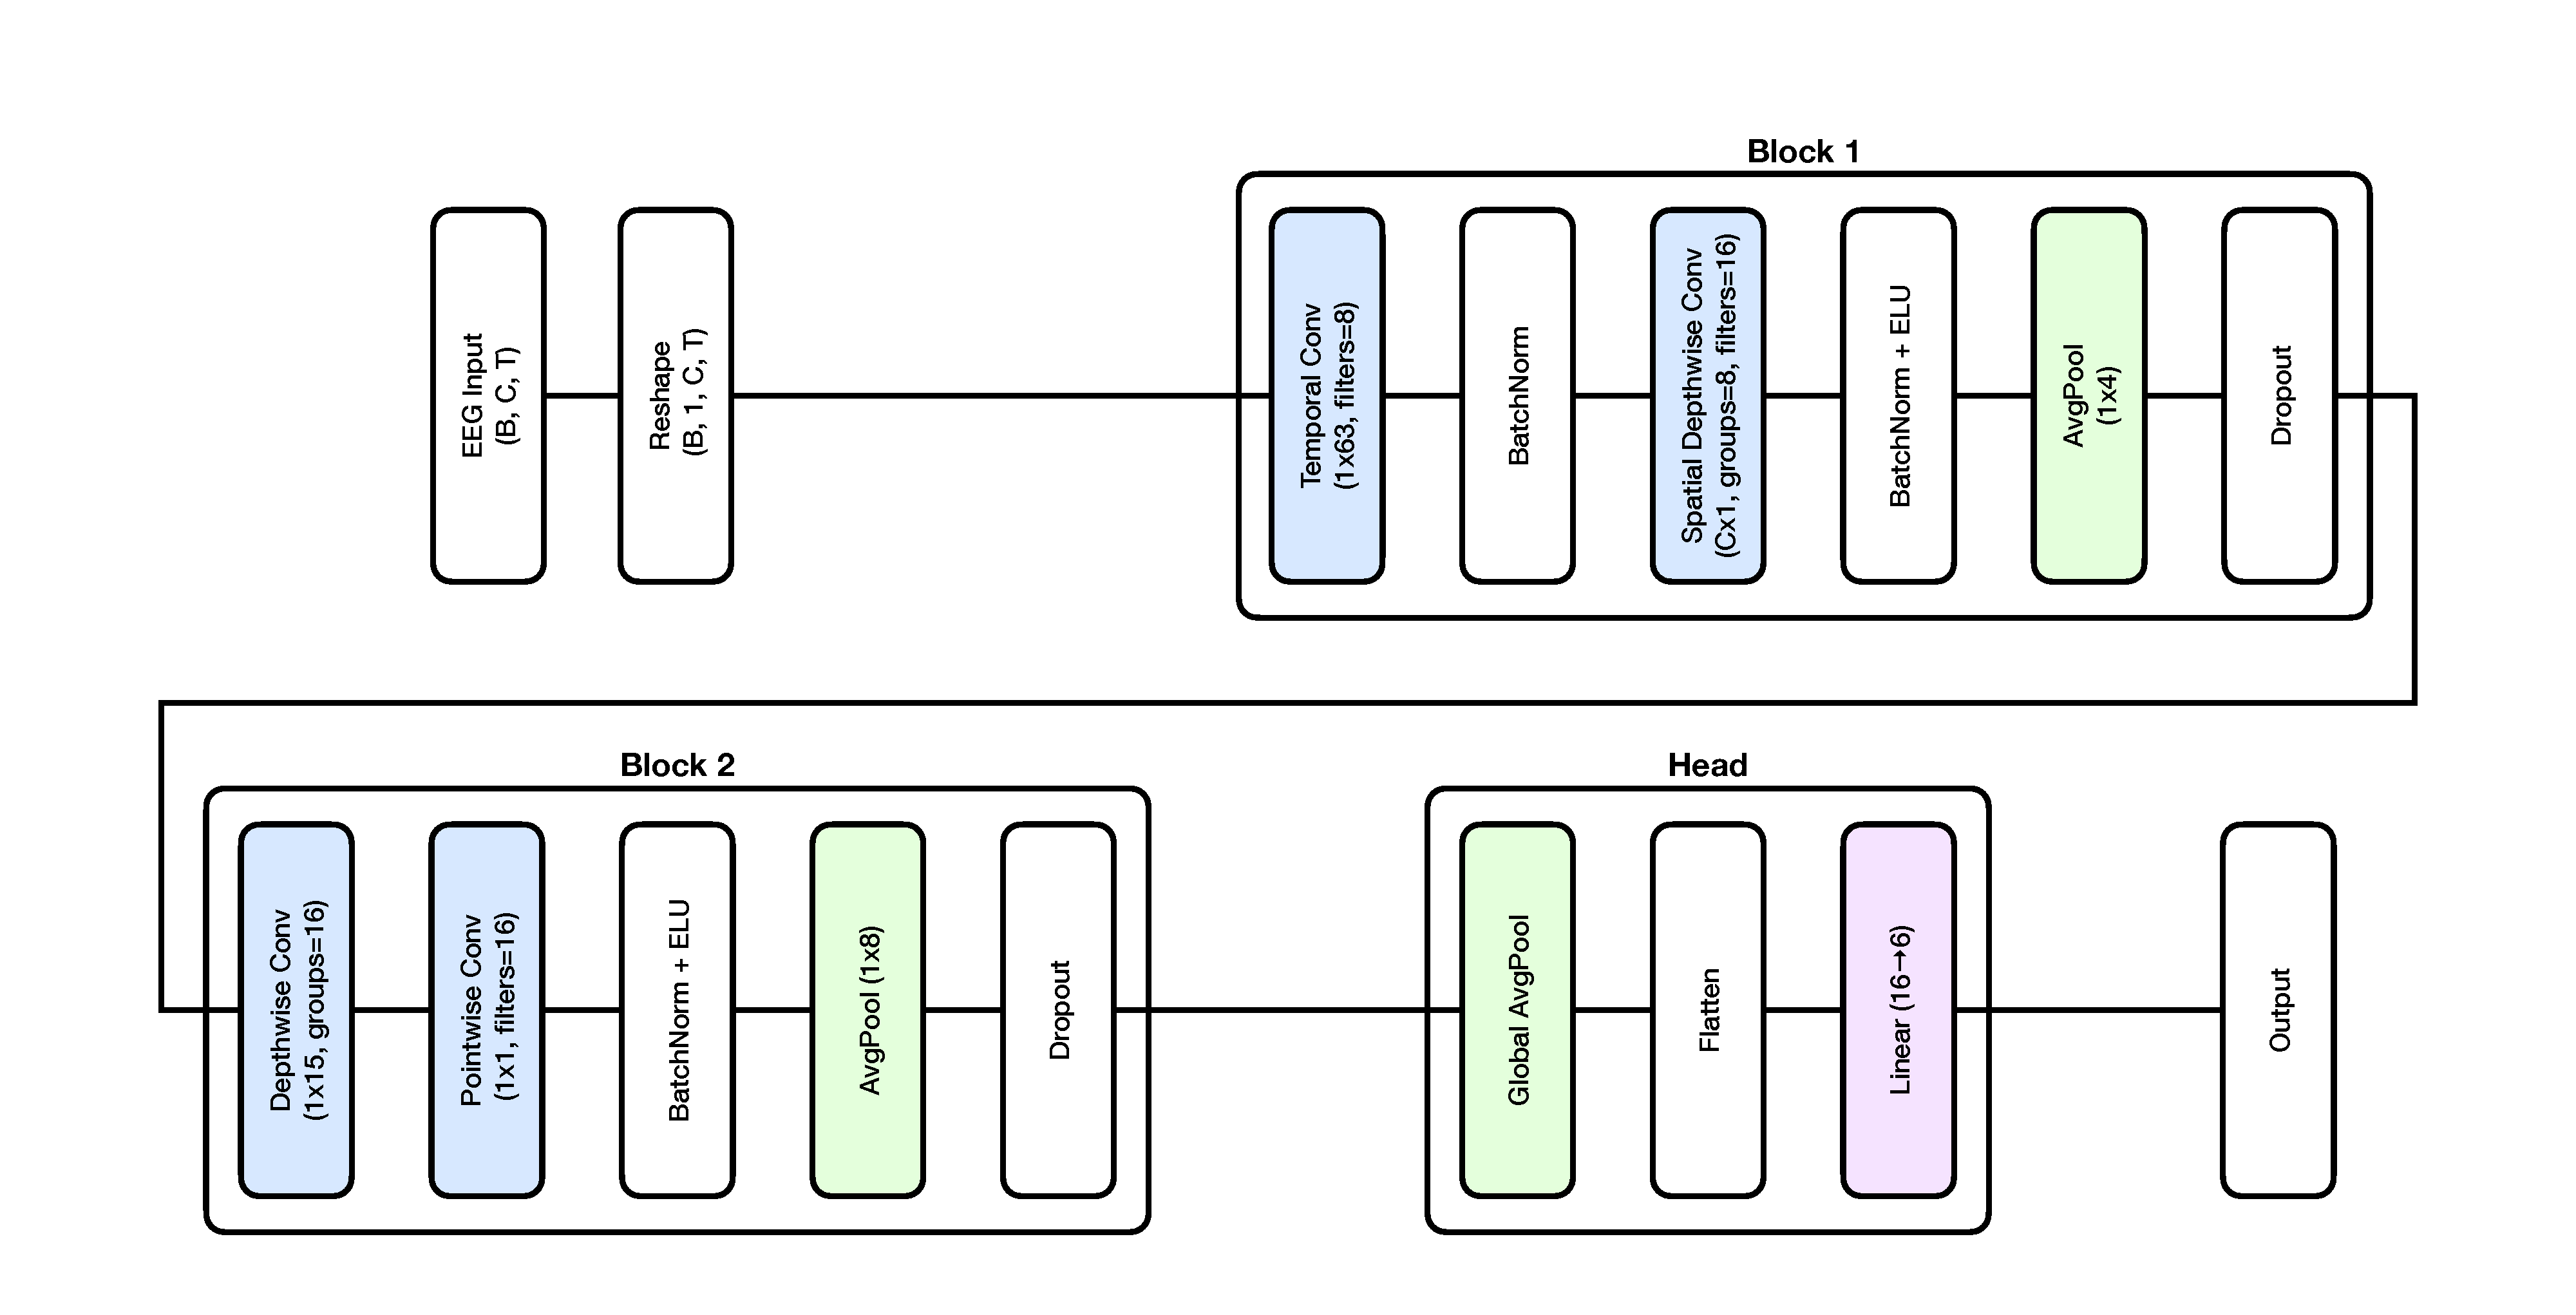
\includegraphics[width=0.9\textwidth]{images/EEGNet.pdf}
    \caption{EEGNet model structure showing Block 1 (temporal extraction and spatial filtering), Block 2 (depthwise temporal refinement), and Head (classification output).}
    \label{fig:EEGNet}
\end{figure}

\subsection{EEGNeX}

EEGNeX \cite{CHEN2024105475} keeps the same goal of learning temporal and spatial structure of the signal as the EEGNet, but it introduces a deeper and more flexible convolutional architecture. EEGNeX is a five-block, convolution only design with two temporal convolution layers, a depthwise spatial convolution across all channels, and two temporal convolutions with dilation. This design makes it capable of capturing long-range temporal dependencies more effectively than its predecessor.

Using multiple temporal convolution layers, the model is able to learn more complex patterns compared to EEGNet which uses only one at the beginning. Another important difference is dilation. Dilated temporal refinement increases the spacing between kernel elements during convolution. The result is a larger temporal context window without an increased kernel size or number of parameters. Batch normalisation is applied after each convolution layer to maintain stable training and dropout is applied after pooling to avoid overfitting.

EEGNeX is a newer architecture that is not as widely adopted as EEGNet, but it has demonstrated competitive performance among CNN-based models for EEG classification tasks.

\begin{figure}[H]
\centering    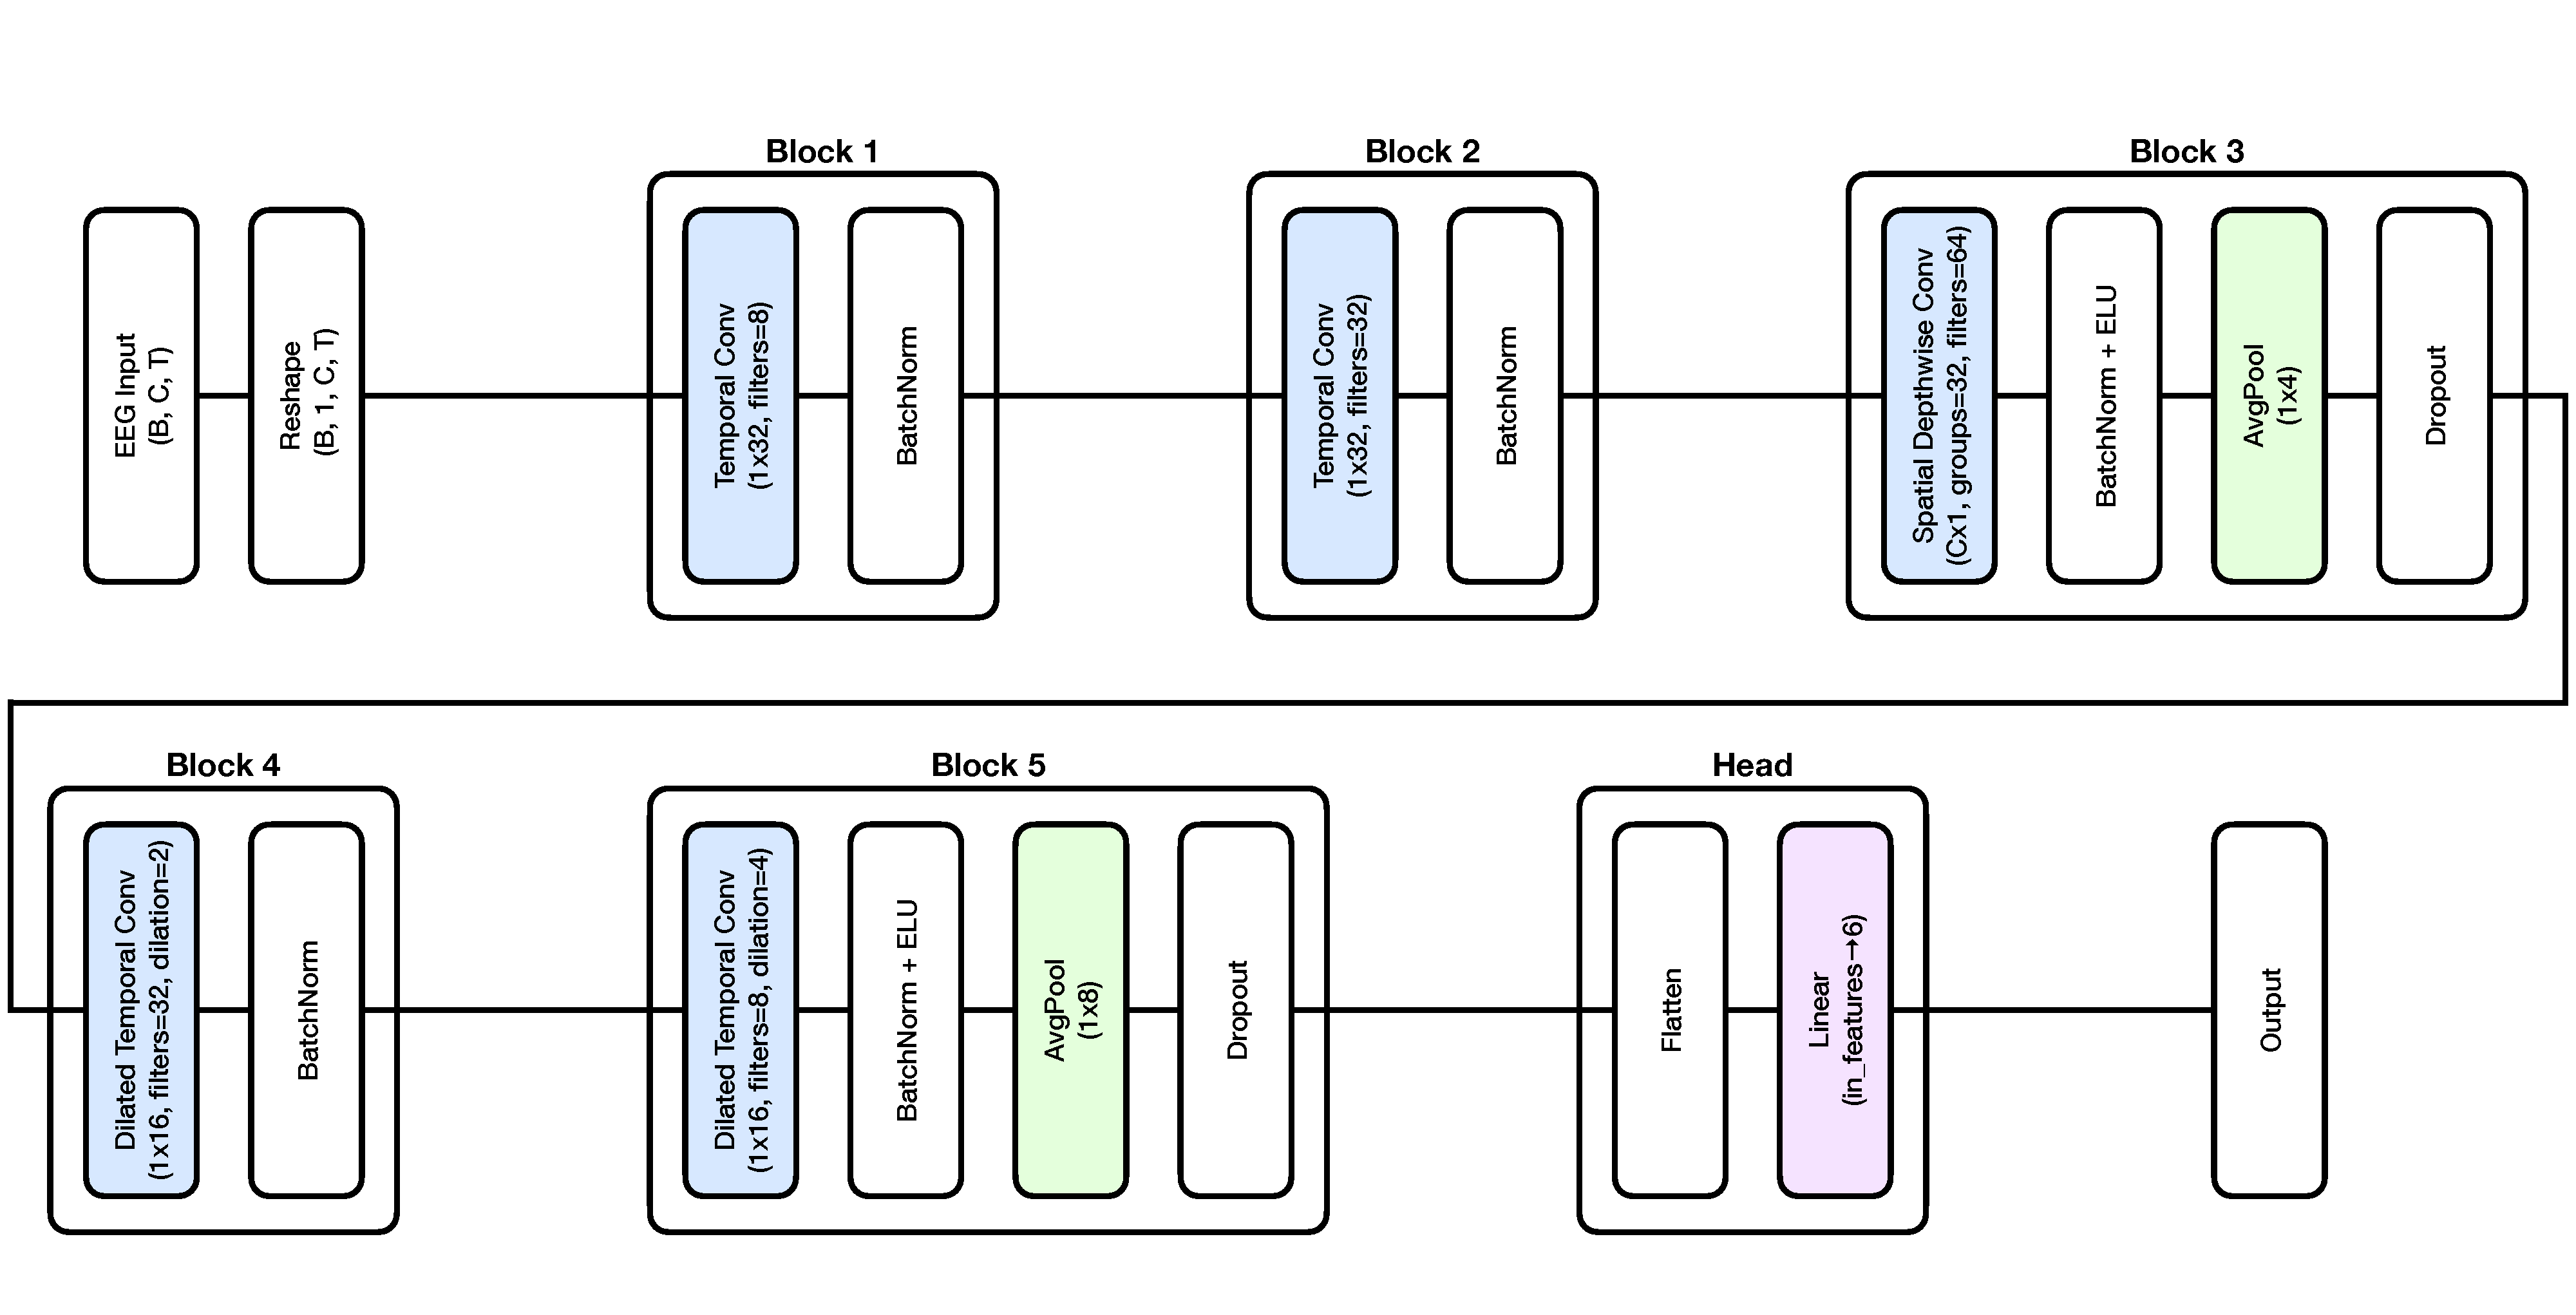
\includegraphics[width=1\textwidth]{images/EEGNeX.pdf}
    \caption{EEGNeX model structure showing Blocks 1-2 (temporal extraction), Block 3 (spatial convolution), Blocks 4-5 (dilated refinement), and Head (classification output).}
    \label{fig:EEGNeX}
\end{figure}

\newpage

\subsection{EEGInceptionERP}

The EEGInceptionERP \cite{EEGInceptionERP} is one of the strongest CNN-based architectures. It extends earlier models by introducing a design that enables multi-scale temporal feature extraction, but remains lightweight compared to other baseline EEG classification models.

The first block contains multi-scale temporal feature extraction and spatial filtering, which are computed on three parallel branches using different kernel sizes. This allows the model to capture both long-term dependencies and short events. The second block refines the extracted features using a similar parallel temporal convolution with smaller kernel sizes, where the goal is to learn finer temporal details of the signal. The third block of the model implements the refinement stage, where convolutions are applied for the extracted feature maps of the previous block followed by the classification head, which produces the output logits corresponding to the target classes.

These components form an efficient and expressive architecture that extends the capabilities of EEGNet and remains more lightweight than EEGNeX.

\begin{figure}[H]
\centering
    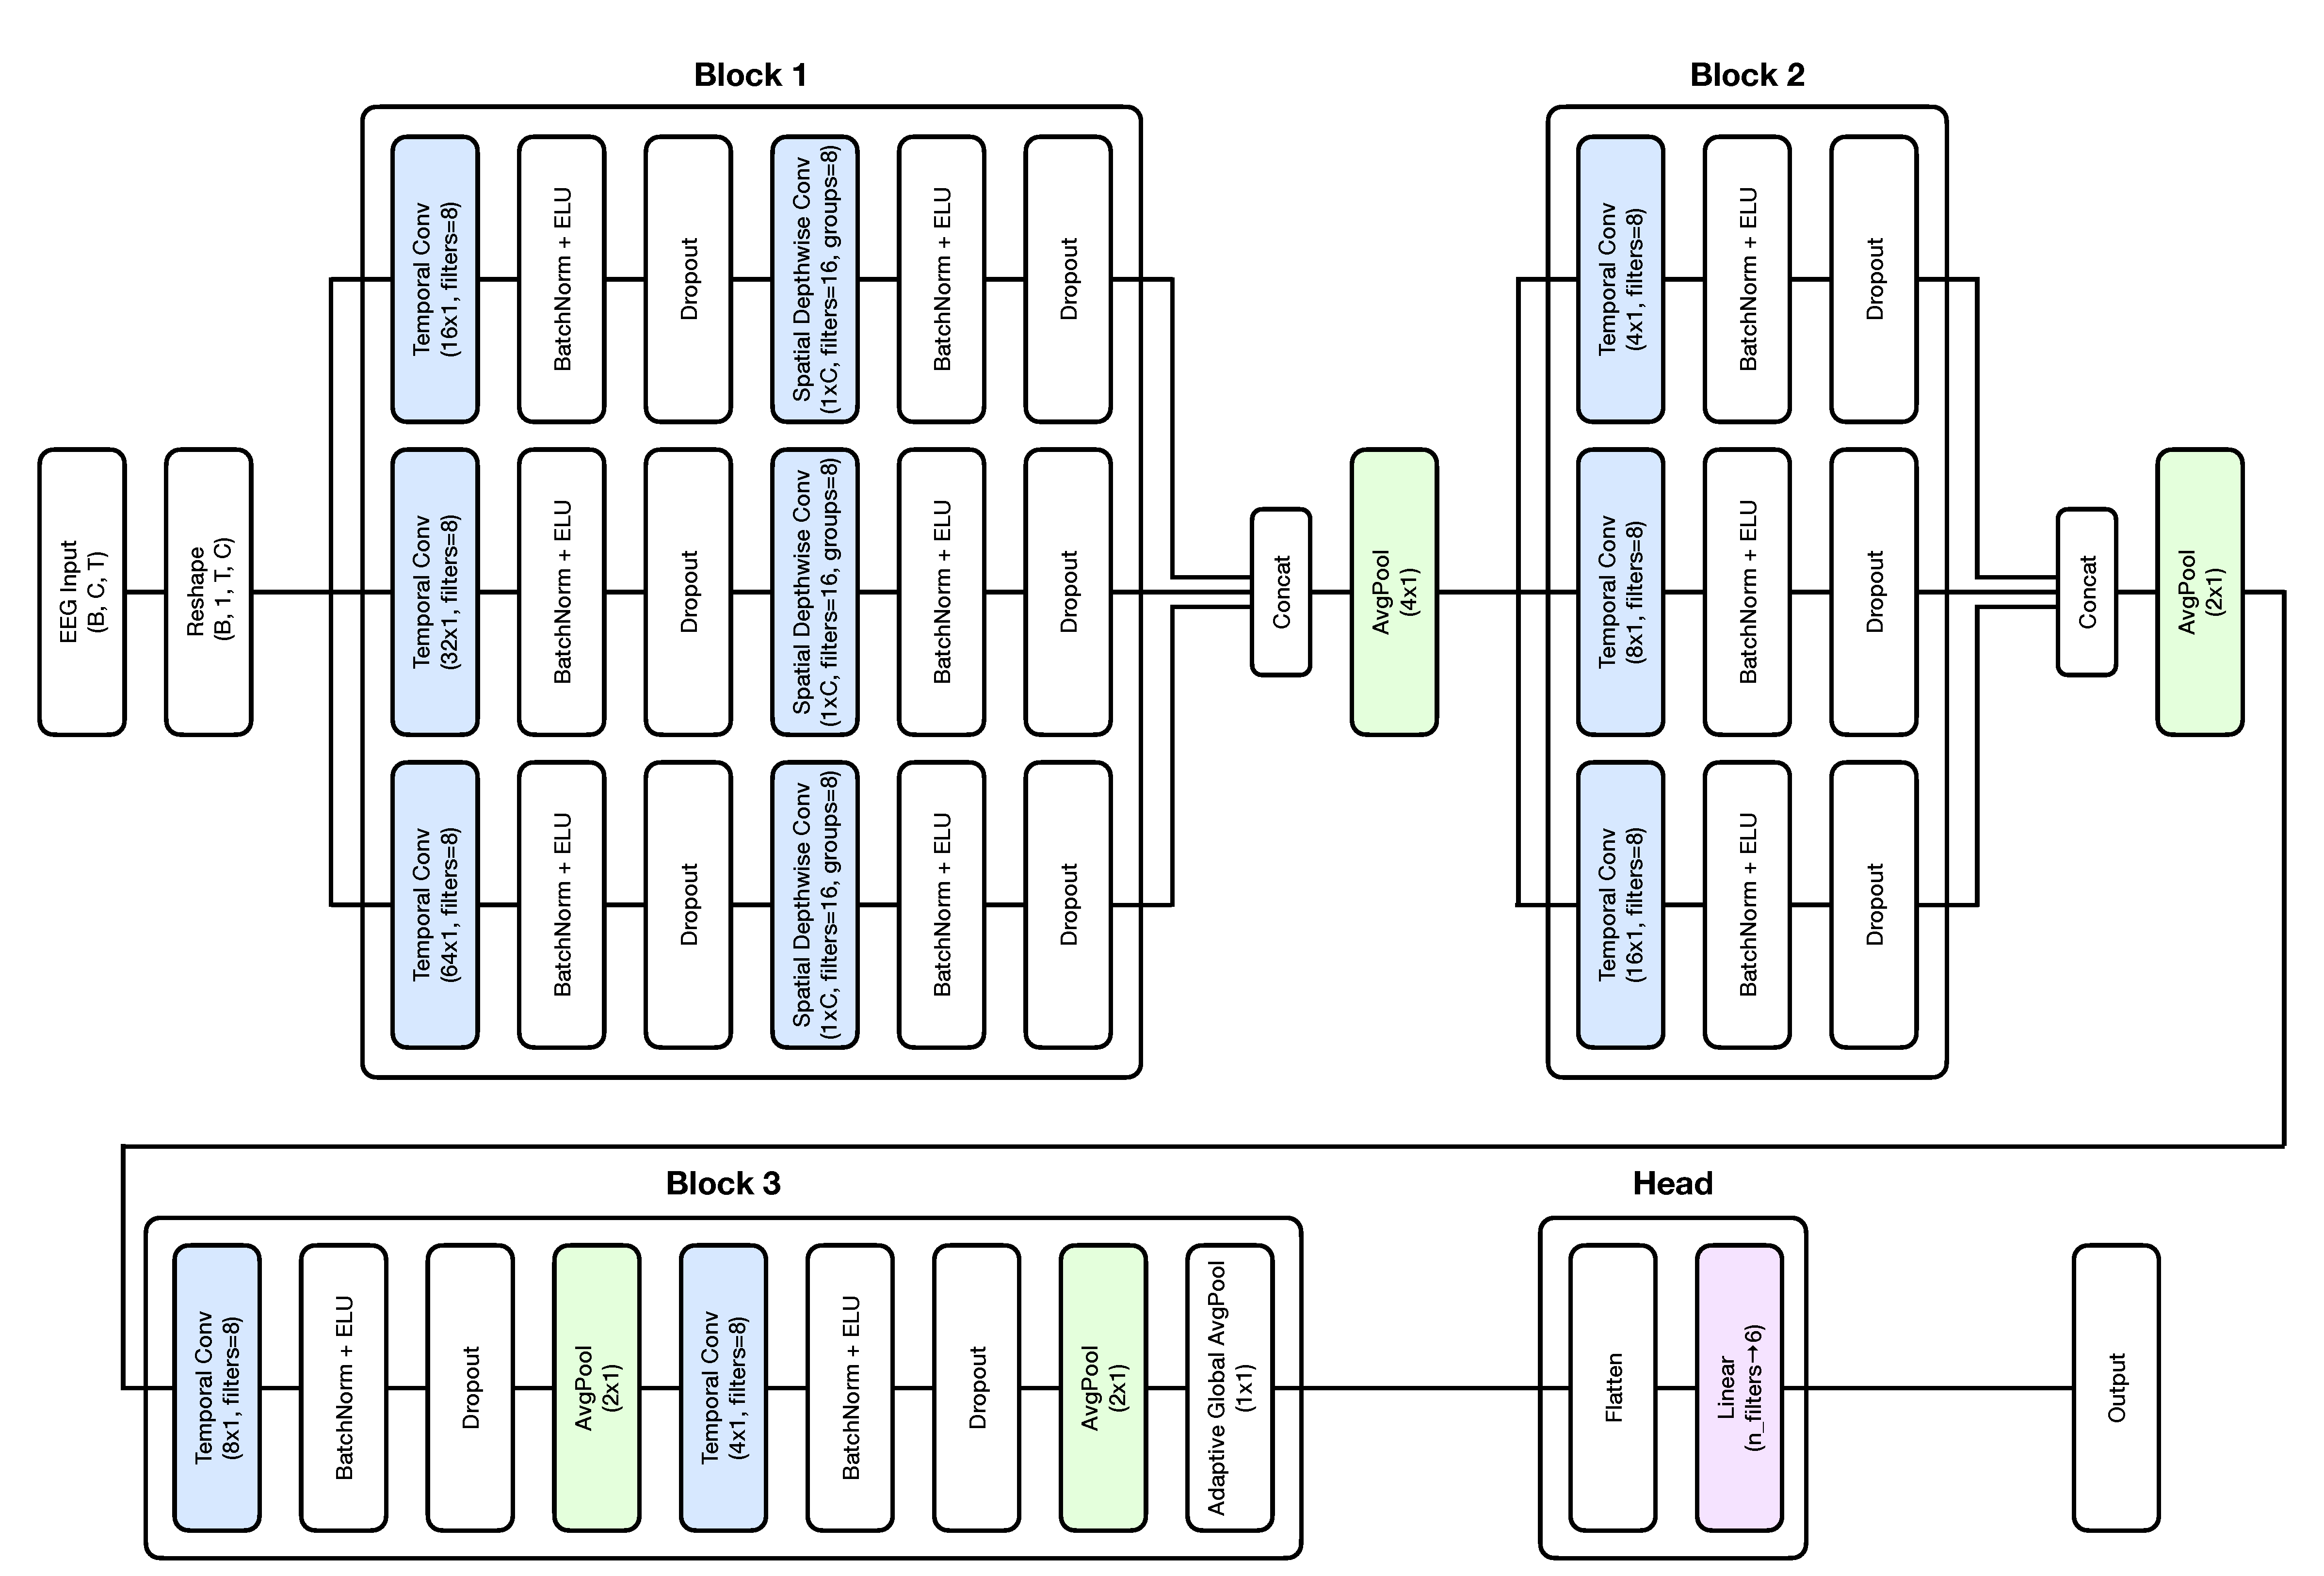
\includegraphics[width=1\textwidth]{images/EEGInceptionERP.pdf}
    \caption{EEGInceptionERP model structure showing Block 1 (multi-scale temporal and spatial extraction), Block 2 (multi-scale temporal refinement), Block 3 (refinement stage), and Head (classification output).}
    \label{fig:EEGInceptionERP}
\end{figure}

\subsection{CNN-LSTM}

This is a CNN-LSTM \cite{inproceedings} hybrid model because it combines convolutional feature extraction with sequence learning methods. It is important to include baseline CNN-RNN models in the experimentation as they serve as an intermediate step between CNN models and more advanced state-of-the-art solutions.

The architecture can be divided into three blocks. The first two blocks contain a 1D convolutional feature extractor similar to EEGNet and EEGNeX, where the EEG channels are treated as input channels of the convolution, and the kernels move only along the time axis. After the two stage CNN part the sequence is passed to the LSTM block that models temporal dependencies in the extracted features, allowing the model to learn contextual information across the entire EEG window segment. In this implementation a bidirectional, multi-layer LSTM is used to allow deeper understanding by processing the sequence in both forward and backward directions. The outputs of the forward and backward passes are combined and the last timestep of the LSTM is selected as the final sequence representation used for classification. This representation is further passed on to the classifier, where the output from the fully connected layer produces logits.

CNN–LSTM architectures have been shown to provide strong performance in EEG classification tasks, outperforming earlier convolutional models while remaining less complex than more advanced approaches. They are also commonly used in practice for time-series and biomedical signal processing tasks due to this balance. For these reasons, this architecture was chosen for the experiments.

\begin{figure}[H]
\centering
    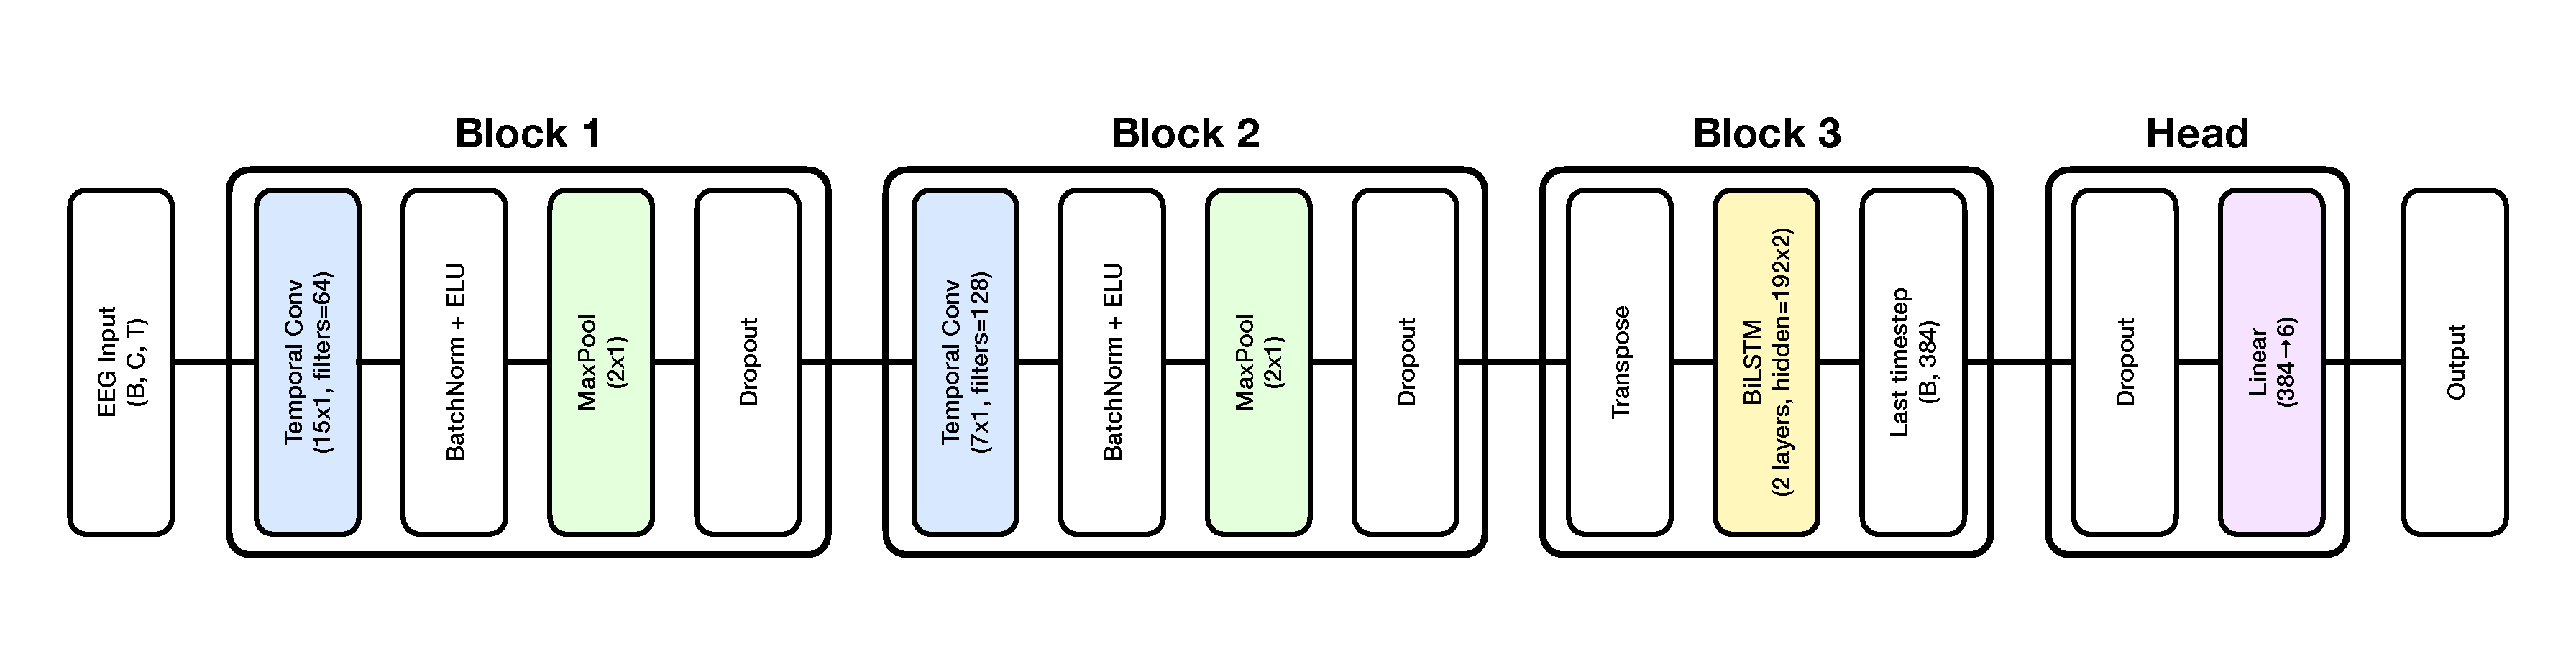
\includegraphics[width=1\textwidth]{images/CNNLSTM.pdf}
    \caption{CNN–LSTM model structure showing Blocks 1–2 (temporal convolutional extraction), Block 3 (bidirectional LSTM sequence modeling), and Head (classification output).}
    \label{fig:CNN-LSTM}
\end{figure}

\subsection{EEGConformer}

EEG-Conformer \cite{Conformer} is a convolution-first model augmented with a lightweight transformer encoder. This hybrid model demonstrated top performance in many EEG signal classification tasks.

The input sequence first passes through the shallow convolutional patch embedding block. A temporal convolution layer captures local temporal patterns along the time axis and a spatial convolution explores relationships between different channels. The second block contains the transformer encoder, where several stacked blocks of multihead attention mechanism and a feed-forward network with skip connections refine the token representations of the signal step by step. This allows the model to capture longer dependencies and global contextual information that cannot be effectively modeled by convolutional operations alone. EEGConformer uses pre-layer normalisation, which means that layer normalisation is applied before the self-attention and feed-forward sublayers as in most modern Transformer designs. The output sequence of the encoder is flattened and passed to final classification head.

This model was included in the set of selected models because of its state-of-the-art performance on many benchmark EEG classification tasks.

\begin{figure}[H]
\centering
    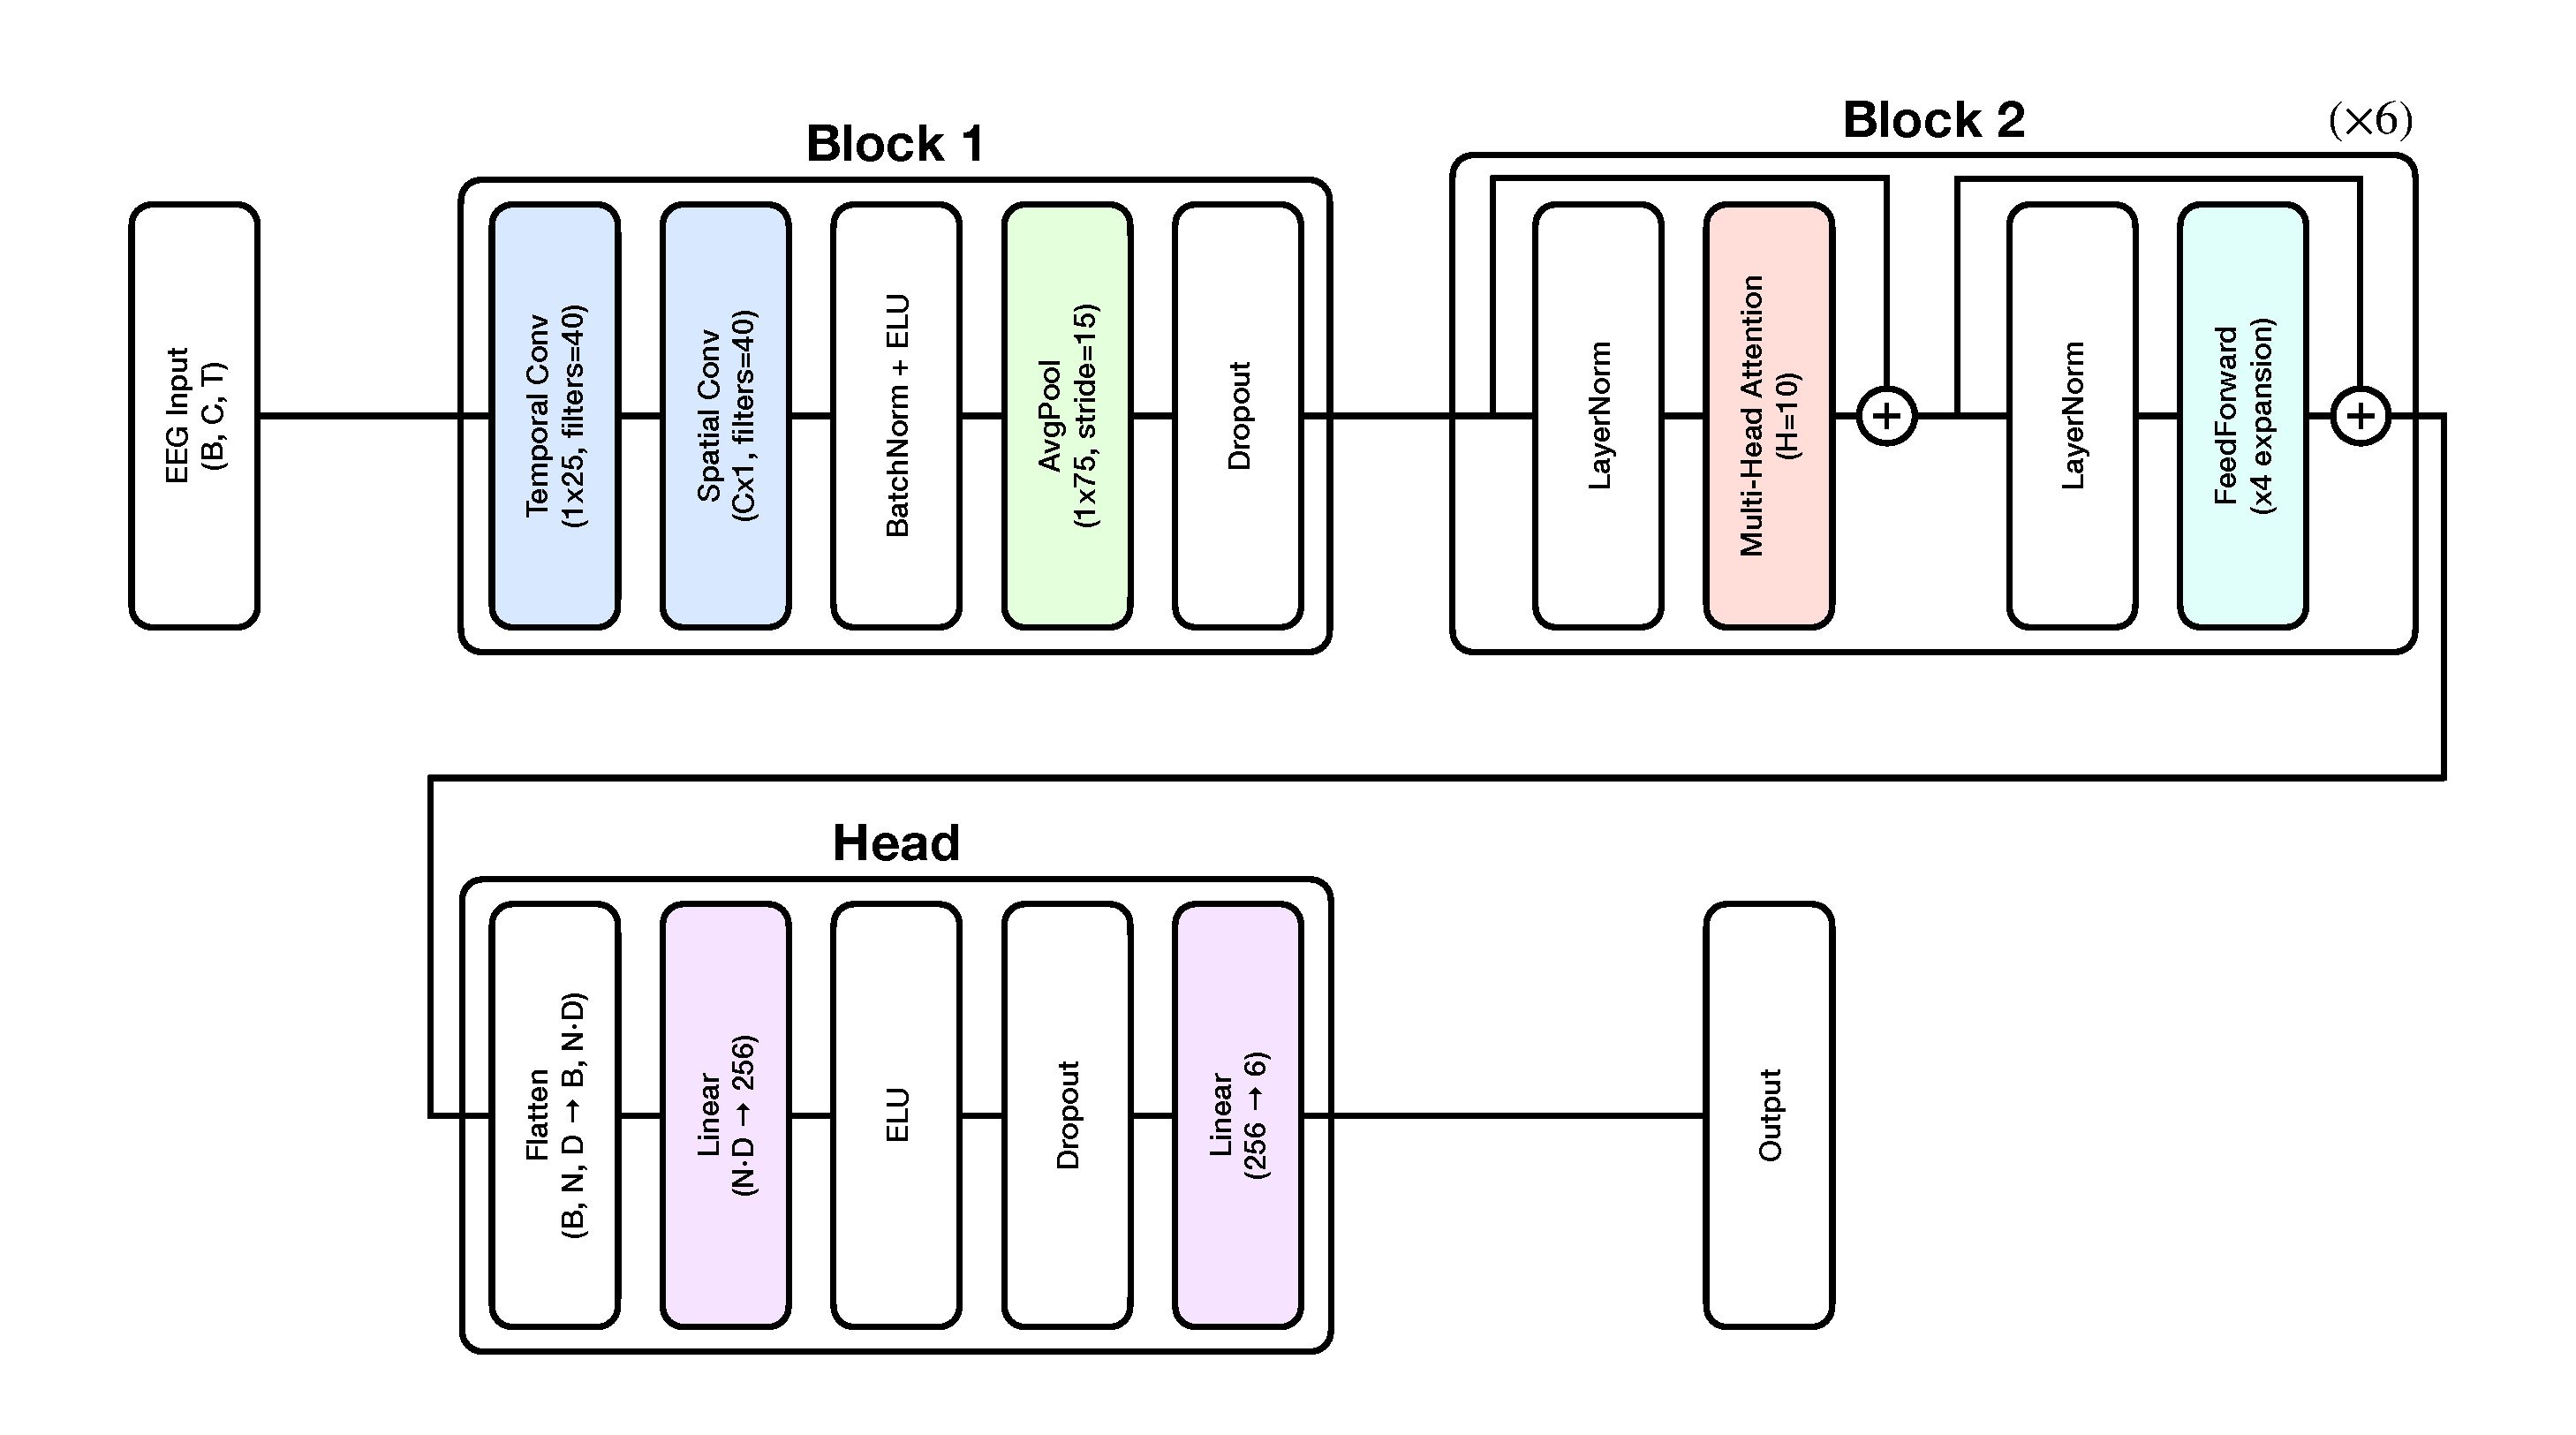
\includegraphics[width=1\textwidth]{images/EEGConformer.pdf}
    \caption{EEGConformer model structure showing Block 1 (temporal and spatial convolutional extraction), Block 2 (multi-head self-attention and feed-forward modeling), and Head (classification output).}
    \label{fig:EEGConformer}
\end{figure}
